\chapter{Theoretical Framework}
\label{chap:theoretical_framework}


This chapter establishes the scientific and engineering foundations required to develop the MONEEE system. It addresses the physiological nature of the signals being measured, the electronic principles of high-precision acquisition, and the computational challenges of synchronizing disparate digital systems.

\section{Neurophysiology \& Event-Related Potentials (ERPs)}
\label{sec:neurophysiology}

Electroencephalography (EEG) measures the electrical activity of the brain via electrodes placed on the scalp. While continuous EEG provides information about the state of the brain (e.g., sleep stages, seizure activity), cognitive neuroscience often focuses on the brain's response to specific sensory, cognitive, or motor events. These time-locked responses are known as Event-Related Potentials (ERPs).

\begin{figure}[h]
    \centering
    % 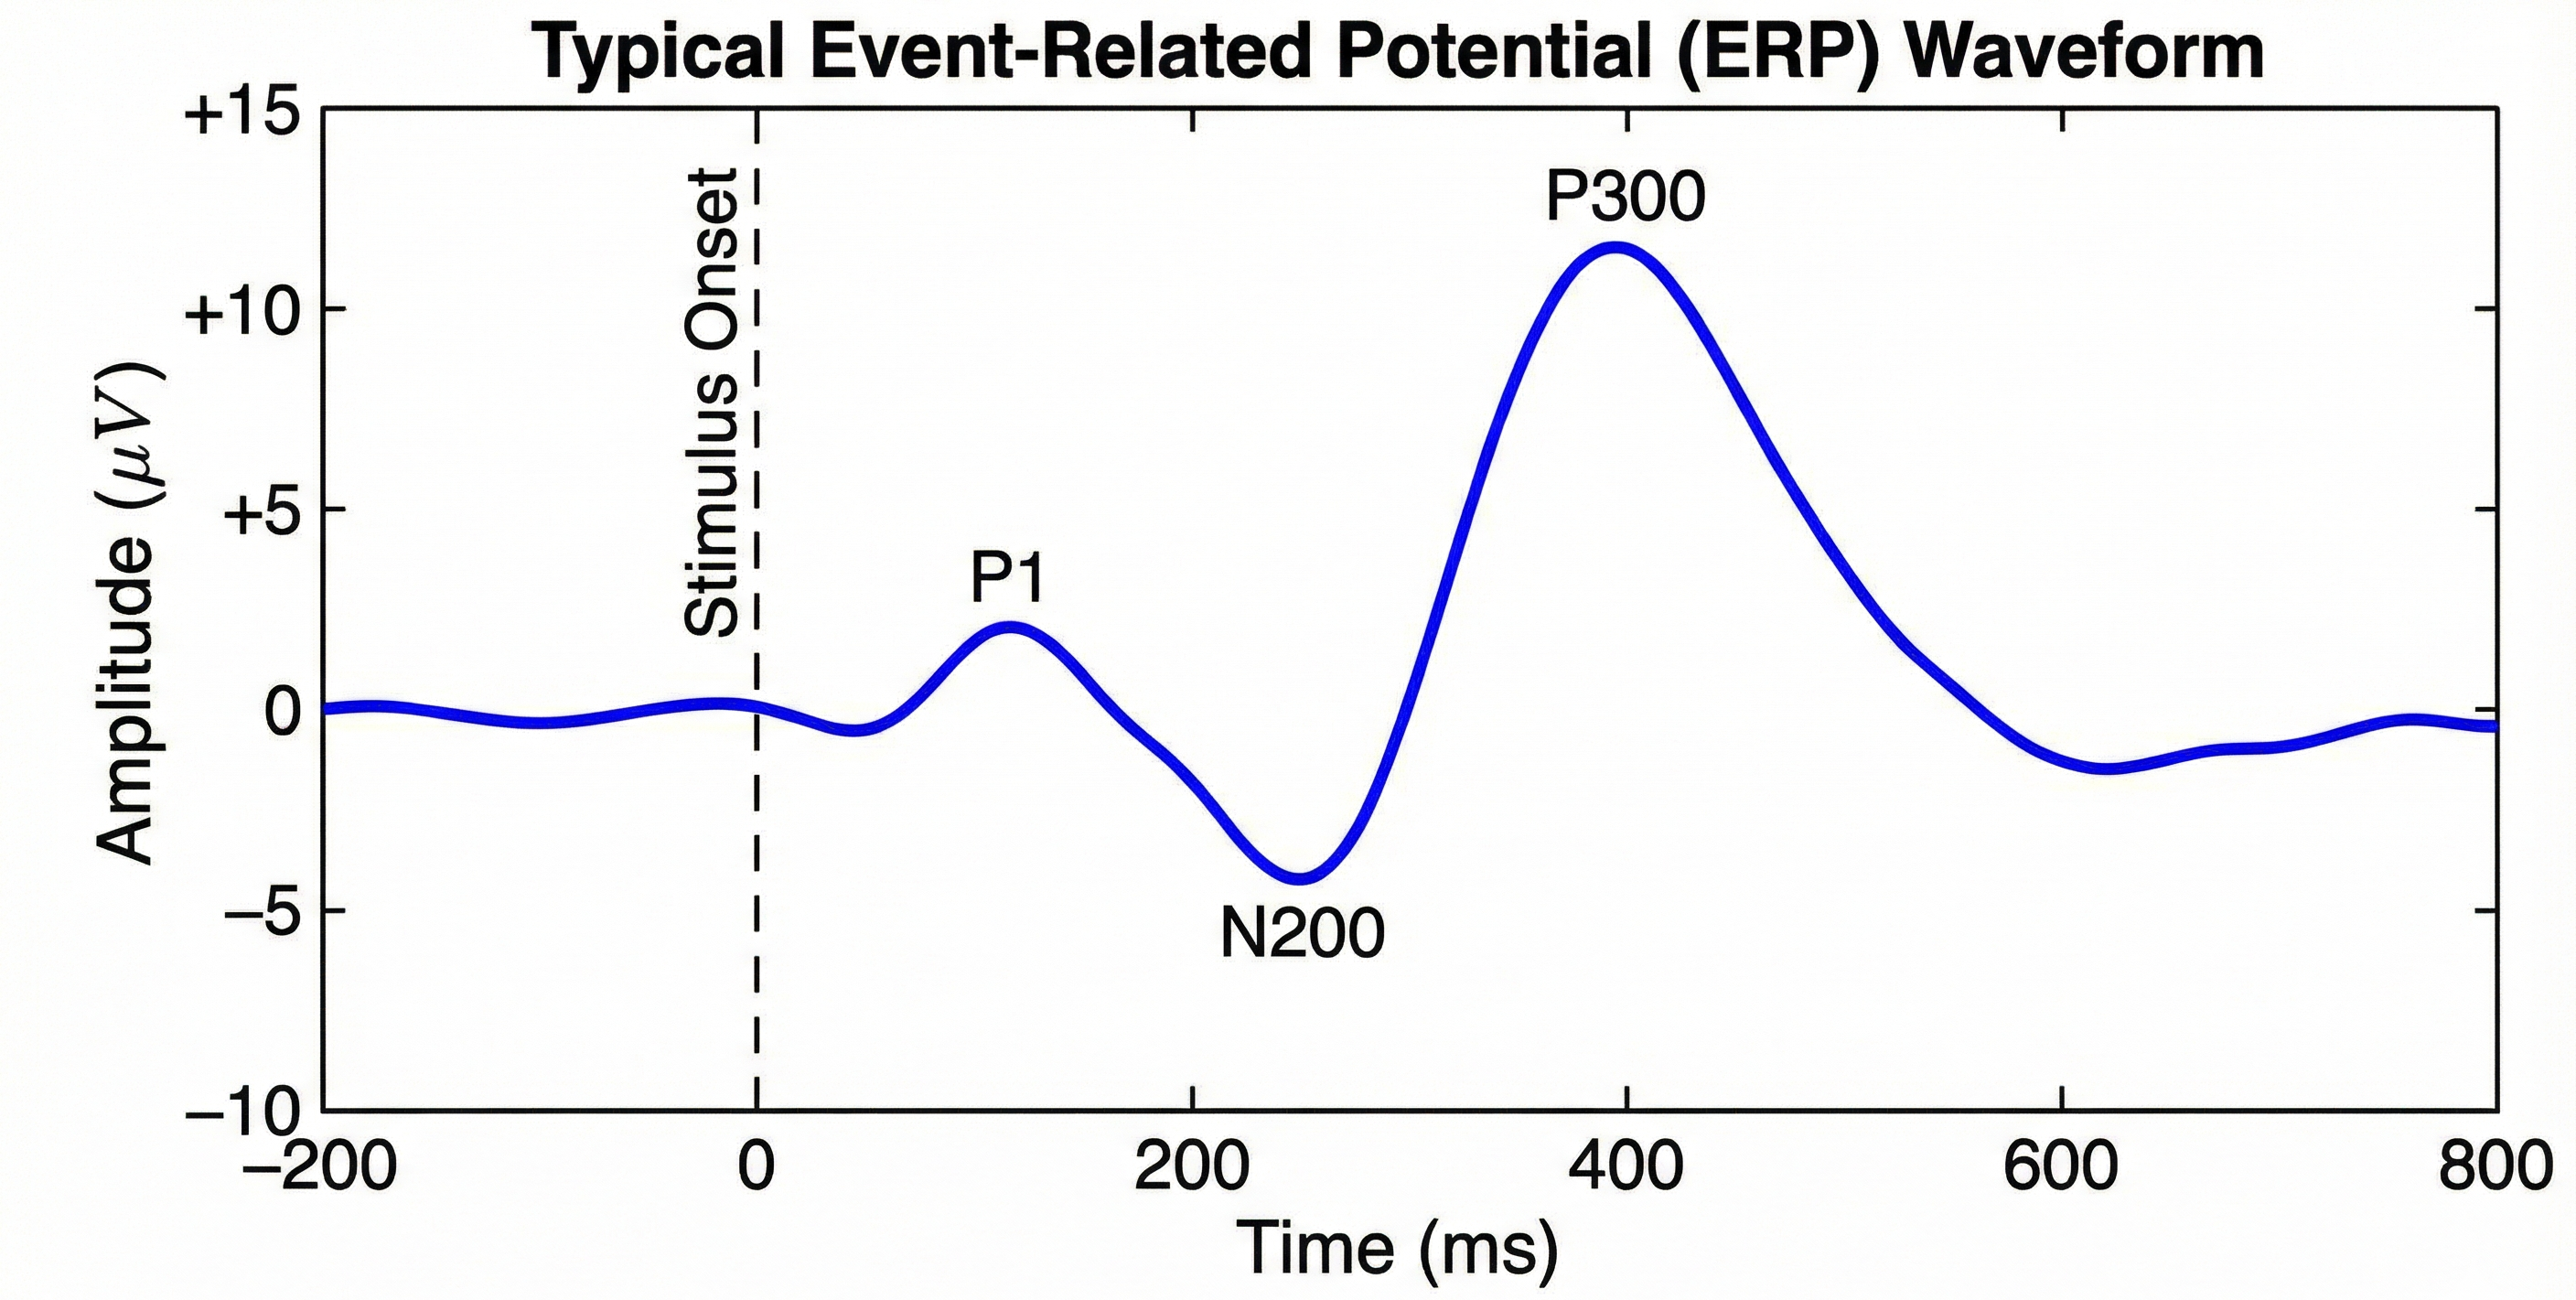
\includegraphics[width=0.8\textwidth]{p300_waveform.png}
    \caption{Typical waveform of an Event-Related Potential showing P300 and N200 components.}
    \label{fig:p300_waveform}
\end{figure}

\subsection{The P300 and N200 Components}
ERPs are small voltage fluctuations (typically $1\mu V$ to $20\mu V$) embedded within the larger background EEG noise ($50\mu V$ to $100\mu V$). Two components are particularly relevant for neurocognitive assessment and serious games:

\begin{itemize}
    \item \textbf{The N200 (N2):} A negative deflection peaking approximately 200--350 ms after stimulus onset. It is primarily associated with executive control functions, specifically mismatch detection (when a stimulus deviates from expectation) and response inhibition.
    \item \textbf{The P300 (P3b):} A large positive deflection peaking 300--600 ms post-stimulus. The P300 reflects processes related to context updating and the allocation of attentional resources. Its amplitude is often proportional to the improbability of the target stimulus (the "oddball" effect), making it a robust metric for assessing attention and cognitive workload in ADHD patients.
\end{itemize}

\subsection{The Necessity of Millisecond-Level Precision}
Because ERPs are much smaller than background brain activity, they cannot be reliably identified in a single trial. Instead, researchers use \textit{Signal Averaging}. By averaging $N$ time-locked trials, the background noise (assumed to be random with a mean of zero) decreases by a factor of $\sqrt{N}$, while the time-locked ERP signal remains constant.

However, this technique relies on the assumption of temporal stability. If the synchronization marker (the "trigger" indicating when the game event occurred) has variable latency—known as \textit{jitter}—the averaging process will "smear" the ERP peaks. Mathematically, if the latency follows a Gaussian distribution with standard deviation $\sigma_t$, the averaged signal is effectively low-pass filtered. A jitter of just $\sigma_t > 10$ ms can significantly attenuate high-frequency components of the N200, rendering the diagnostic data invalid. Therefore, the MONEEE system requires hard-real-time synchronization capabilities.

\section{Signal Acquisition Hardware}
\label{sec:hardware}

The fidelity of the EEG data depends heavily on the analog-front-end architecture. The MONEEE system utilizes the Texas Instruments ADS1299, a specialized Analog-to-Digital Converter (ADC) for biopotential measurements.

\subsection{Delta-Sigma ($\Delta\Sigma$) Analog-to-Digital Converters}
Unlike Successive Approximation Register (SAR) ADCs often found in general-purpose microcontrollers, the ADS1299 is a Delta-Sigma modulator. This architecture is chosen for its superior noise performance and dynamic range.

\begin{enumerate}
    \item \textbf{Oversampling:} The ADC samples the input at a frequency ($f_{mod}$) much higher than the Nyquist rate. This spreads the quantization noise over a wider bandwidth.
    \item \textbf{Noise Shaping:} The modulator pushes the quantization noise into higher frequencies, away from the biological signal band (0--100 Hz).
    \item \textbf{Digital Filtering:} A subsequent digital decimation filter removes the high-frequency noise and reduces the data rate to the user-selected output (e.g., 250 SPS or 500 SPS).
\end{enumerate}

\begin{figure}[h]
    \centering
    % \includegraphics[width=0.8\textwidth]{delta_sigma_block.png}
    \caption{Simplified block diagram of a Delta-Sigma ADC architecture.}
    \label{fig:delta_sigma}
\end{figure}

\subsubsection{Simultaneous Sampling}
A critical feature of the ADS1299 is its ability to sample all 8 channels simultaneously. In multiplexed architectures, a single ADC switches between channels sequentially, introducing a phase delay between electrodes ($t_{skew}$). For EEG connectivity analysis (coherence), $t_{skew}$ must be zero. The ADS1299 achieves this by dedicating a separate $\Delta\Sigma$ modulator to every channel.

\subsection{Heterogeneous Embedded Systems: MCU vs. MPU}
To balance signal integrity with data throughput, modern acquisition systems often employ a heterogeneous architecture, combining a Microcontroller Unit (MCU) and a Microprocessor Unit (MPU).

\begin{itemize}
    \item \textbf{The MCU (e.g., TM4C1294):} Acts as the hard real-time controller. It operates "bare metal" or with a Real-Time Operating System (RTOS). Its primary role is \textbf{determinism}. When the ADC indicates data is ready (via a \texttt{DRDY} hardware interrupt), the MCU must capture it within microseconds to prevent FIFO overflows. It is responsible for timestamping the incoming data precisely when it arrives.
    \item \textbf{The MPU (e.g., Raspberry Pi Compute Module):} Runs a rich Operating System like Linux. It handles high-throughput tasks such as network stacks (TCP/IP), file storage, and complex drivers. However, standard Linux is non-deterministic; the kernel scheduler may preempt a task for 10--20 ms to handle background processes.
    \item \textbf{The Synergy:} In the MONEEE architecture, the MCU guarantees the timing of the acquisition, effectively isolating the sensitive bio-signals from the non-deterministic jitter of the Linux-based MPU.
\end{itemize}

\section{Digital Synchronization Protocols}
\label{sec:sync_protocols}

Synchronizing the EEG data (recorded by hardware) with the game events (generated by software) is the principal challenge of this thesis. Several methods exist, each with trade-offs regarding latency and intrusiveness.

\begin{table}[h]
    \centering
    \caption{Comparison of Synchronization Methods}
    \label{tab:sync_methods}
    \begin{tabular}{p{3cm} p{5cm} p{2.5cm} p{3.5cm}}
        \toprule
        \textbf{Method} & \textbf{Mechanism} & \textbf{Precision} & \textbf{Implementation} \\
        \midrule
        Optical (Photodiode) & Hardware sensor detects pixel changes on screen. & High ($<1$ ms) & High (External hardware required). \\
        Network (LSL) & Time-sync via NTP-like protocols over LAN. & Medium ($<5$ ms) & Low (Software only). \\
        Hardware Trigger (TTL) & Parallel port or USB-to-TTL directly to ADC. & Very High ($<1$ ms) & Medium (Legacy ports or dongles). \\
        \bottomrule
    \end{tabular}
\end{table}

\subsection{Optical vs. Network Synchronization}
\textbf{Optical (Ground Truth):} Placing a photodiode on the monitor to detect the exact moment a visual stimulus appears. This bypasses all operating system and GPU rendering delays. It is often used as the "gold standard" to validate other methods but is impractical for widespread clinical deployment due to the hardware setup required.

\textbf{Lab Streaming Layer (LSL):} A network-based middleware that handles time-series data. It synchronizes streams by mapping local machine timestamps to a common clock, performing jitter correction. While effective, it relies on the quality of the local network and the accuracy of the software timestamps generated by the game engine.

\subsection{USB Latency Characteristics}
The MONEEE system utilizes USB for communication between the MCU and the MPU/Host. Understanding USB latency is vital for "soft-triggers" (commands sent from the PC to the amplifier).

\begin{itemize}
    \item \textbf{Polling Intervals:} USB is a host-controlled bus. The host polls the device for data.
    \begin{itemize}
        \item \textit{Full Speed (USB 2.0):} Frame time is 1 ms. Data is transferred only once per frame.
        \item \textit{High Speed:} Microframe time is $125 \mu s$.
    \end{itemize}
    \item \textbf{CDC Class Overhead:} The Communication Device Class (CDC) emulates a serial port. While convenient for development, the OS driver stack buffers data to improve throughput, often at the cost of latency. A command sent by the game engine may sit in the OS output buffer for several milliseconds before being placed on the USB bus (Start-of-Frame), creating variable delays inconsistent with ERP analysis requirements.
\end{itemize}
